\section{Second Order Partial Differential Equations}
\hrule
\noindent\\
\subsection{The Heat and Wave Equations}
\indent Let's take a look at the second order PDE. We will start with a
homogeneous equation, which we will tackle with the separation of variables
method. The general strategy is that we want to take our PDE and convert it to
an ODE, which we know how to solve. The problems presented here also involve
boundary conditions, which will require us to solve for eigenvalues/functions.
We will also be dealing with series (specifically Fourier Series) to help us
solve these problems. Let's look at an example:\\
\noindent\textbf{\textit{Ex:}} Solve the following boundary value problem:
\[
\begin{cases}
u_{tt} - u_{xx} = 0\\
u(0,t) = 0\qquad u(1,t) = 0\\
u(x,0) = f(x)\qquad u_{t}(x,0) = g(x)
\end{cases}\\
\]
\[f(x) = 2\sin{(\pi x)} + 3\sin{(2\pi x)}\qquad g(x) = 4\sin{(3\pi x)} - 7\sin{(5\pi x)}\]
given the general solution:
\[u(x,t) = \sum_{n=1}^{\infty}\left[\left(a_{n}\cos{[n\pi t]} + b_{n}\sin{[n\pi t]}\right)\sin{[n\pi
x]}\right]\]
\indent\textbf{\textit{Solution:}} There's a lot going on here, so let's break
it down. First of all, notice that we have two initial conditions, one of which
is a derivative. This should make sense since the equation have two second order
partial derivatives included in it. Next notice that we have a Fourier Sine Series,
despite both the $\sin{[n\pi t]}$ and $\cos{[n\pi t]}$ terms. If we had worked
out the entire problem, we would see that our eigenvalue/function for this
equation takes the form of
\[
\{\lambda_{n} = n\pi, \sin{(n\pi x)}\}
\]
\noindent which tells us that the corresponding series is a Fourier Sine Series.
We also see the initial conditions on our equation are already representative
of a series of sine functions, which is not just a conincidence. To apply the
initial conditions, we will need both the general solution and the derivative
with respect to $t$ of the general solution. Let's go ahead and apply the first
initial condition, $u(x,0) = f(x)$. Letting $t= 0$ gives us:
\[
u(x,0) = 2\sin{(\pi x)} + 3\sin{(2\pi x)} = \sum_{n=1}^{\infty}\left[a_{n}\sin{(n\pi x)}\right]
\]
\noindent We see that the term with $b_{n}$ has dropped out, since
$\sin{(0)} = 0$. Now we just have to match up the coefficients on $a_{n}$. We
can see that when we have $n=1$, $a_{n} = 2$, and when $n=2$, $a_{n} = 3$. For
all other $n$, we have $a_{n} = 0$, so we ignore those terms. Next, we can apply
the initial condition for the derivative of the general solution with respect to
$t$. We expect that all the terms related to $a_{n}$ will disappear, and in fact
they will. Let's take a look:
\begin{align*}
u_{t}(x,t) &= \sum_{n=1}^{\infty}\left[(-a_{n}n\pi\sin{[n\pi t]} + b_{n}n\pi\cos{[n\pi t]})\sin{n\pi
x}\right]\\
u_{t}(x,0) &= 4\sin{(3\pi x)} - 7\sin{(5\pi x)} = \sum_{n=1}^{\infty}\left[n\pi b_{n}\sin{(n\pi
x)}\right]
\end{align*}
\noindent We are going to do the same thing here that we did to find our $a_{n}$
terms, but notice that we don't just have $b_{n}$; we actually have $n\pi b_{n}$.
We have the following:
\begin{alignat*}{3}
&3\pi b_{3} = 4 \qquad \qquad \qquad &&5\pi b_{5} = -7\\
&b_{3} = \frac{4}{3\pi} &&b_{5} = -\frac{7}{5\pi}
\end{alignat*}
\noindent Much like the solutions for $a_{n}$, all the other $b_{n}$ terms are 0.
Now we can construct a particular solution. In this case, the answer will not be
in the form of a series, since we have definite terms. Our solution is as follows:
\[
u(x,t) = 2\cos{(\pi t)}\sin{(\pi x)} + 3\cos{(2\pi t)}\sin{(2\pi x)} + \frac{4}{3\pi}\sin{(3\pi
t)}\sin{(3\pi x)} - \frac{7}{5\pi}\sin{(5\pi t)}\sin{(5\pi x)}
\]
\noindent And we are done.
\newpage

\noindent \textbf{\textit{Ex:}} Solve the following PDE
\[
\begin{cases}
\frac{\partial u}{\partial t} = k \frac{\partial^{2} u}{\partial x^{2}}\\
u(x,0) = x\\
u(0,t) = u(L,t) = 0\\
\end{cases}
\]
\indent \textbf{\textit{Solution:}} We will use the separation of variable
technique to solve this problem. We know to use separation of variable because
we are dealing with a homogeneous PDE with homogenous boundary conditions.
Separation of variables tells us that our solution will be in the form of
$u(x,t) = X(x)T(t)$. If we take this fact at face value, we can use the
separation of variables method to solve this. First, we substitute in our solution
into the PDE:
\begin{align*}
\frac{\partial}{\partial t}(X(x)T(t)) &= k \frac{\partial^{2}}{\partial x^{2}}(X(x)T(t))\\
X(x)\frac{dT}{dt} &= k\frac{d^{2}X}{dx^{2}}T(t)\\
\frac{dT}{dt}\frac{1}{T(t)} &= \frac{d^{2}X}{dx^{2}}\frac{k}{X(x)}
\end{align*}
\noindent The only way that our function of x and our function of t can be equal
is if they are equal to a constant; thus we now have:
\[
\frac{dT}{dt}\frac{1}{T(t)} = \frac{d^{2}X}{dx^{2}}\frac{k}{X(x)} = -\lambda
\]
\noindent And now we have a first order ODE for the time and a second order ODE
for the position:
\[
\frac{dT}{dt} = -k \lambda T(t) \qquad\text{and}\qquad \frac{d^{2}X}{dx^{2}} = -\lambda X(x)
\]
\noindent Our next step is to find the Eigenvalues and Eigenfunctions of the
second order ODE; we will come back to the time ODE when we have values for
$\lambda$.\\
\indent To solve for these values, we have to find non-trivial eigenvalues that
correspond to the boundary values of the ODE. In this case, we know that
$X(0) = 0$ and $X(L) = 0$. These boundary conditions come from the BC on the PDE
which states $u(0,t) = u(L,t) = 0$. To find the eigenvalues/functions, we need
to find the characteristic equation corresponding to the ODE in question. Let's
go ahead and find it:
\begin{gather*}
\frac{d^{2}X}{dx^{2}} = -\lambda \frac{X(x)}{k}\\
\frac{d^{2}X}{dx^{2}}  + \lambda \frac{X(x)}{k} = 0\\
r^{2} + \lambda = 0\\
r^{2} = -\lambda\\
r = \pm \sqrt{- \lambda}
\end{gather*}
\indent Now, we can substitute values of $\lambda$ to find out solutions. Let's
start with $\lambda > 0$. Since we have a $-\lambda$ under the radical, we will
have $r = \pm \sqrt{\lambda} \mathrm{i}$. This will yield the solution of
\[
y(x) = c_{1}\cos{\sqrt{\lambda}x} + c_{2}\sin{\sqrt{\lambda}x}
\]
\noindent Applying our boundary conditions gives us:
\[
y(0) = c_{1}\cos{0} + c_{2}\sin{0} = 0
\]
\noindent Now we know that $c_{1} = 0$. This result came from the fact that
$\sin{0} = 0$, so the $c_{2}$ term disappears. Now we are left with $\cos{0} = 1$,
which tells us that $c_{1} = 0$. We can apply this to our second boundary
condition like so:
\begin{gather*}
y(L) = 0 = c_{2}\sin{\sqrt{\lambda}L}\\
\end{gather*}
\noindent It looks like there will only be trivial solutions, but we know this
isn't true due to the Jacobian matrix. Recall that if the determinant of the
Jacobian $\neq 0$, then we only have trivial solutions, and if the determinant
of the Jacobian $= 0$, then we do not have the trivial solution. Let's take a
look at the Jacobian for this case:
\begin{gather*}
\left|
\begin{array}{cc}
1 & 0\\
\cos{\sqrt{\lambda}L} & \sin{\sqrt{\lambda}L}
\end{array}
\right| = 0\\
\sin{\sqrt{\lambda}L} = 0\\
\sqrt{\lambda}L = \arcsin{0}\\
\sqrt{\lambda} = \frac{\arcsin{0}}{L}\\
\lambda = \left(\frac{\arcsin{0}}{L}\right)^{2}\\
\lambda = \left(\frac{n\pi}{L}\right)^{2}
\end{gather*}
\noindent Notice that we replaced the $\arcsin{0}$ term with $n\pi$. Recall from
trig that the $\sin$ function is $0$ at every $n\pi$, starting with $n = 0$.
Next, we just need to find our corresponding eigenfunction. Our $c_{1}$ was $0$,
so we can ignore the entire $\cos$ term. Thus, we have an eigenfunction from
plugging in our $\lambda$ that looks like:
\[
X(x) = \sin{\frac{n\pi x}{L}}
\]
\indent Unfortunately, we aren't done yet. Now we have to find the corresponding
eigenvalues/functions for $\lambda = 0$. This isn't too hard, and can be done in
a few lines if we recall the characteristic equation. Plugging in $0$ for
$\lambda$ gives us that $r = 0$. Using this piece of information, we now know
that $y(x) = c_{1} + xc_{2}$. Applying our boundary conditions gives us
$c_{1} = 0, c_{2} = 0$. We can see that we have only trivial solutions for
$\lambda = 0$.\\
\indent Our final case is for $\lambda < 0$. I'll go ahead and tell you that
this will yield another trivial solution, but we can take a look at the work
behind it. Since $\lambda > 0$, we know that our $r$ from the characteristic
equation will be $r = \pm \sqrt{\lambda}$. From here we are going to do something
 a little unconventional that will help us. Usually, we would have a solution of
the form $y(x) = c_{1}e^{\sqrt{\lambda}x} + c_{2}x e^{-\sqrt{\lambda}x}$. In our
case, it will be more convenient to use hyperbolic trig functions. It's not too
far off from our solution from $\lambda > 0$:
\begin{align*}
y(x) &= c_{1}e^{\sqrt{\lambda}x} + c_{2}e^{-\sqrt{\lambda}x}\\
&= c_{1}\cosh{\sqrt{\lambda}x} + c_{2}\sinh{\sqrt{\lambda}x}
\end{align*}
\noindent If we apply the boundary conditions (remember that
$\sinh{0} = 0$ and $\cosh{0} = 1$), we will find that we have only trivial
solutions.\\
\indent So, we are done with the second order ODE, and now we turn our eye to
the first order time equation. We know our $\lambda$, so it isn't too hard to solve:
\begin{gather*}
\frac{dT}{dt} = -\lambda T(t)\\
T(t) = ce^{-k\left(\frac{n\pi}{L}\right)^{2}t}
\end{gather*}
\indent Finally we can put it all together. Our penultimate solution will be
\[
u_{n}(x,t) = B_{n}\sin{\left(\frac{n\pi x}{L}\right)}e^{-k\left(\frac{n\pi}{L}\right)^{2}t}
\]
\noindent We can analyze this solution and tell where each piece comes from.
The $B_{n}$ is a coefficient that results from our $c's$ in the general solutions
of the differential equations. The $sin$ part results from out eigen vector.
Remember, we get a different value for each $n$, so there may or may not be $0$
terms in the series. Finally, we have the exponential term. This term comes from
the solution to our time equation. When we put it all together, we can see that
this is, of course a series; for every $n$, we get a different solution. From
here we can find the Fourier Series (which will be a Fourier Sine Series). We
won't worry about that yet, but we will come back to it.
\newpage


\indent It will benefit us to take a moment and discuss how boundary conditions
effect our Fourier series. We have three different combinations of boundary
conditions, where each one will produce a different result in our series solution.
\begin{enumerate}
\item \textit{Dirichlet Boundary Conditions}\\
Dirichlet boundary conditions involve the function for which we are looking. In
other words, the boundary conditions are presented in terms of the functions we
are trying to find, rather than the derivative of that function. Typically, this
type of boundary condition will take the form of (in the homogeneous case)
\[u(0,t) = u(L,t) = 0.\]
In regards to our Fourier series, we expect to see $\sin{(\frac{n\pi x}{L})}$.
Our basis will look like
\[
\left\{ \lambda_{n} = \left(\frac{n\pi}{2}\right)^{2}, \phi_{n}(x) = \sin{\left(\frac{n\pi x}{L}\right)}
\right\}
\]
\item \textit{Neumann Boundary Conditions}\\
Neumann boundary conditions involve the derivatives of the function for which we
are solving. Neumann boundary conditions will look like
\[u_{x}(0,t) = u_{x}(L,t) = 0.\]
This will cause our Fourier series to contain $\cos{(\frac{n\pi x}{L})}$. Our
basis will look like
\[
\left\{ \lambda_{n} = \left(\frac{n\pi}{2}\right)^{2}, \phi_{n}(x) = \cos{\left(\frac{n\pi x}{L}\right)}
\right\}
\]
\item \textit{Robin Boundary Conditions}\\
Robin boundary conditions will contain a mixture of the function and it's
derivative. Typically, we will see
\[ u_{x}(0,t) = u(L,t) = 0\qquad \text{or}\qquad u(0,t) = u_{x}(L,0) = 0.\]
These boundary conditions will give us two different results, depending on whether
we have the derivative first or second. We will have
\begin{align*}
u_{x}(0,t) = u(L,t) = 0 &\implies \left\{\lambda_{n} = \left(\left[n +
\frac{1}{2}\right]\frac{\pi}{L}\right)^{2}, \phi_{n}(x) = \cos{\left(\left[n +
\frac{1}{2}\right]\frac{\pi}{L}x\right)}\right\}\\
u(0,t) = u_{x}(L,t) = 0 &\implies \left\{\lambda_{n} = \left(\left[n +
\frac{1}{2}\right]\frac{\pi}{L}\right)^{2}, \phi_{n}(x) =\sin{\left(\left[n +
\frac{1}{2}\right]\frac{\pi}{L}x\right)}\right\}
\end{align*}
\end{enumerate}

\indent Now we can take a look at a slightly harder PDE. We still have the heat
equation, but we will not have homogeneous boundary conditions. Our goal here is
to find a way to transform our boundary conditions into a homogenous form and take
it from there.\\\\
\noindent \textbf{\textit{Ex:}} Solve the following PDE
\[
\begin{cases*}
u_{t} - u_{xx} = 0\\
u(0,t) = 0,\ u(1,t) = t\\
u(x,0) = x^{2}
\end{cases*}
\]
\indent \textbf{\textit{Solution:}} We would like to just jump into this PDE and
solve it, but it's not quite that simple. We have to find a way to express our
boundary conditions in a homogeneous manner. We can do this through a clever
substitution; we will create a new PDE, denoted $\Upsilon$. To find $\Upsilon$,
we use the following formula:
\[ \Upsilon = B_{1} + \frac{x}{l}\Delta B, \]
\noindent where $B$ is a boundary condition. In our case, we have as follows:
\begin{align*}
\Upsilon &= B_{1} + \frac{x}{l}\Delta B\\
&= 0 + \frac{x}{1}(t - 0)\\
&= xt
\end{align*}
\noindent Now, we find a new PDE, denoted by $\upsilon$. We have another formula that tells us
\[ \upsilon(x,t) = u(x,t) - \Upsilon(x,t) \]
\noindent Applying this formula gives us
\begin{align*}
\upsilon(x,t) &= u(x,t) - \Upsilon\\
&= u(x,t) - xt
\end{align*}
\noindent Let's take a moment to analyze the result. We wanted to find a new PDE in terms of our old one
that would allow us to have homogeneous boundary conditions. We found a solution, called $\upsilon$, in
terms of our original PDE, called $u$. Our original PDE was $u_{t} - u_{xx} = 0$, so to properly perform
our substitution, we need to find $\upsilon_{t}$ and $\upsilon_{xx}$. Through some careful
differentiation, we have
\[ \upsilon_{t} = u_{t} - x \qquad\text{and}\qquad \upsilon_{xx} = u_{xx}\]
\noindent To find our new PDE, we simply evaluate.
\[
\upsilon_{t} - \upsilon_{xx} = u_{t} - x - u_{xx} = u_{t} - u_{xx} - x = 0 - x = -x
\]
\noindent So we finally have a new PDE that looks like
\[
\begin{cases*}
\upsilon_{t} - \upsilon_{xx} = -x\\
\upsilon(0,t) = \upsilon(1,t) = 0\\
\upsilon(x,0) = x^{2}
\end{cases*}
\]
\noindent You may wonder how this has made anything simpler, since the PDE itself is no longer
homogeneous. By forcing the boundary conditions to be homogeneous, we can now use a Fourier series to
find our solution. Recall that earlier we discussed the boundary condition and their resulting
eigenvalue/eigenfunction. Here, we have Dirichlet boundary conditions, which tells us that we have a
Fourier sine series. We have that
\begin{align*}
\upsilon(x,t) &= \sum_{n = 1}^{\infty}\left[a_{n}(t)\sin{(n\pi x)}\right]\\
\upsilon_{t}(x,t) &= \sum_{n = 1}^{\infty}\left[a_{n}'(t)\sin{(n\pi x)}\right]\\
\upsilon_{xx}(x,t) &= -\sum_{n = 1}^{\infty}\left[a_{n}(t)(n\pi)^{2}\sin{(n\pi x)}\right]\\
\end{align*}
\noindent Which tells us that
\[
\upsilon_{t} - \upsilon_{xx} = \sum_{n = 1}^{\infty}\left[(a_{n}'(t) + (n\pi)^{2}a_{n}(t))\sin{(n\pi
x)}\right] = -x
\]
\noindent This may look rather complicated, but all we have is a function's Fourier sine series.
Essentially, we have
\[
-x = \sum_{n = 1}^{\infty}\left[ b_{n}\sin{(n\pi x)} \right]
\]
\noindent To find $b_{n}$, we use the formula that was discussed in the earlier section about Fourier
series. We have that
\begin{align*}
a_{n}'(t) + (n\pi)^{2}a_{n}(t) &= \int_{0}^{1}-x\sin{(n\pi x)}dx\\
&= \frac{2x}{n\pi}\cos{(n\pi x)}\bigg\vert_{0}^{1}\\
&= \frac{2}{n\pi}
\end{align*}
\noindent We now have an ODE which we can solve for $a_{n}$. Note that from out PDE, we do have an
initial condition for the ODE, but it is not as simple as just saying $a_{n}(0) = x^{2}$. At $t = 0$, we
have the following series:
\[
\sum_{n=1}^{\infty} a_{n}(0)\sin{(n\pi x)}
\]
\noindent We got this by taking our original $\upsilon(x,t)$ and plugging in $0$ for $t$. We know how to
get $a_{n}(0)$, since this is just a simple Fourier sine series. It is given by
\begin{align*}
a_{n}(0) &= 2\int_{0}^{1}x^{2}\sin{(n\pi x)}dx\\
&= \frac{(-1)^{(n + 1)}}{n\pi} + \frac{2}{(n\pi)^{3}}\left[ (-1)^{n} - 1 \right]
\end{align*}
\noindent We now have all we need to solve the ODE. We will omit the work for the solution, but the
final answer for $a_{n}$ is
\[
a_{n}(t) = \frac{4\left[ (-1)^{n} - 1 \right]}{(n\pi)^{3}}e^{-(n\pi)^{2}t} +
\frac{2(-1)^{n}}{(n\pi)^{3}}
\]
\noindent Now all that's left to do is go back to $u$ from $\upsilon$. This may seem hard, but we saw earlier that $\upsilon = u - \Upsilon$. Solving for $u$ gives us $u = \upsilon + \Upsilon$. Recall that $\Upsilon$ was $xt$, and $\upsilon$ was the series for which we just found $a_{n}$. Putting it all together gives us
\[
u(x,t) = xt + \sum_{n=1}^{\infty}\left[\frac{4\left[ (-1)^{n} - 1 \right]}{(n\pi)^{3}}e^{-(n\pi)^{2}t} + \frac{2(-1)^{n}}{(n\pi)^{3}}\right]\sin{(n\pi x)}
\]
\noindent And we are done.
\newpage


\noindent \textbf{\textit{Ex:}} Solve the following PDE
\[
\begin{cases*}
u_{tt} - u_{xx} = 1 + t\cos{(2\pi x)}\\
u_{x}(0,t) = u_{x}(1,t) = 0\\
u(x,0) = 2\cos{(2\pi x)},\quad u_{t}(x,0) = 1 + \cos{(\pi x)} - \cos{(2\pi x)}
\end{cases*}
\]
\indent \textbf{\textit{Solution:}} This problem is an example of the wave equation with a non-homogeneous solution. We are lucky this time; the boundary conditions are already homogeneous, so there is no need to change our variable. We know that since both of the boundary conditions are derivatives, we are dealing with a Fourier cosine series. This yields the eigenvalue/function of
\[
\left\{\lambda_{n} = (n\pi)^{2}, \cos{(n\pi x)}\right\}
\]
Since we are dealing with a cosine series, we also have a leading term, $a_{0}$. Our full series looks like
\[
u(x,t) = a_{0}(t) + \sum_{n=1}^{\infty} a_{n}(t)\cos{(n\pi x)}
\]
We need $u_{tt}$ and $u_{xx}$, so we have:
\[
u_{tt}(x,t) = a_{0}''(t) + \sum_{n=1}^{\infty} a_{n}''(t)\cos{(n\pi x)}
\qquad \text{and} \qquad
u_{xx}(x,t) = -\sum_{n=1}^{\infty} (n\pi)^{2}a_{n}(t)\cos{(n\pi x)}
\]
All we have to do now is simply plug into our original equation. This gives us
\begin{align*}
a_{0}''(t) + \sum_{n=1}^{\infty} a_{n}''(t)\cos{(n\pi x)} + \sum_{n=1}^{\infty} (n\pi)^{2}a_{n}(t)\cos{(n\pi x)} &= 1 + t\cos{(2\pi x)}\\
a_{0}''(t) + \sum_{n=1}^{\infty}(a_{n}''(t) + (n\pi)^{2}a_{n}(t))\cos{(n\pi x)} &= 1 + t\cos{(2\pi x)}
\end{align*}
Now we can play the matching game. We have a $constant + series\ term$ on the right side, and $constant + series$ on the left, so we can match up the constants. This gives us
\[
a_{0}''(t) = 1
\]
Now we match up the series term. On the right hand side, we have $\cos{(2\pi x)}$, so we know that for $n= 2$, we have
\[
a_{2}''(t) + 4\pi^{2}a_{2}(t) = t
\]
$a_{0}$ and $a_{2}$ are the only terms that appear, so we can assume for now that $\forall n \neq 2\ \text{and}\ 3, a_{n} = 0$. We are left with two ODE's, so we now need to find the corresponding initial conditions. Let's apply the first initial condition to our PDE. This gives us
\[a_{0}(0) + \sum_{n=1}^{\infty}a_{n}(0)\cos{(n\pi x)} = 2\cos{(2\pi t)}\]
Which tells us
\[a_{0} = 0 \qquad\qquad \qquad\qquad a_{2} = 2\]
Now we can apply the second initial condition. After taking the partial derivative of $u$ with respect to $t$, we have
\[
a_{0}'(0) + \sum_{n=1}^{\infty}a_{n}'(0)\cos{(n\pi x)} = 1 + \cos{(\pi x)} - \cos{(2\pi x)}
\]
Some more clever pattern matching give us
\[
a_{0}'(0) = 1 \qquad\qquad a_{1}'(0) = 1 \qquad\qquad a_{2}'(0) = -1
\]
Notice that we have a term $a_{1}'$. We cannot simply ignore this value; rather we have to take it into account when we find our solution. We know that we have an ODE for $a_{1}(t)$, but it may not be evident how to express it. Recall that earlier we said $\forall n \neq 2\ \text{and}\ 3, a_{n} = 0$. This means that $a_{1} = 0$, and since $a_{1}$ is a coefficient in the Fourier series, we know that $a_{1}''(t) + \pi^{2}a_{1}(t) = 0$. We now have three different ODE's that we must solve:
\begin{alignat*}{3}
&\begin{cases}
a_{0}''(t) = 1\\
a_{0}'(0) = 1,\quad a_{0}(0) = 1
\end{cases}
&\begin{cases}
a_{1}''(t) + \pi^{2}a_{1}(t) = 0\\
a_{1}'(0) = 1,\quad a_{1}(0) = 0
\end{cases}
&&\begin{cases}
a_{2}''(t) + 4\pi^{2}a_{2}(t) = t\\
a_{2}'(0) = 1,\quad a_{2}(0) = 2
\end{cases}
\end{alignat*}
Luckily, Mathematica is here to save the day. We will skip the work and let the computer do the thinking for us. We get that
\begin{align*}
a_{0}(t) &= \frac{1}{2}t^{2} + t\\
a_{1}(t) &= \frac{\pi\cos{(t\pi)} + \sin{(t\pi)}}{\pi}\\
a_{2}(t) &= \frac{2\pi t + 16\pi^{3}\cos{(2\pi t)} - \sin{(2\pi t)} + 4\pi^{2}\sin{(2\pi t)}}{8\pi^{3}}
\end{align*}
Now all we need to do is plug back in to our $u$. Our final answer becomes
\[
u(x,t) = \frac{1}{2}t^{2} + t + \frac{\pi\cos{(t\pi)} + \sin{(t\pi)}}{\pi}\cos{(\pi x)} +  \frac{2\pi t + 16\pi^{3}\cos{(2\pi t)} - \sin{(2\pi t)} + 4\pi^{2}\sin{(2\pi t)}}{8\pi^{3}}\cos{(2\pi x)}
\]
Just for interest, the plot of this solution looks like
\begin{center}
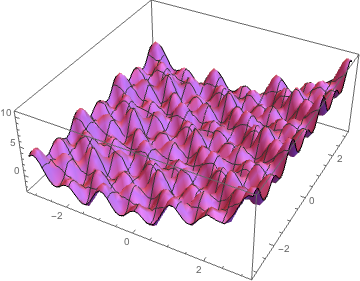
\includegraphics[scale=0.6]{pg23_plot}
\end{center}
On $-\pi \leq \theta \leq \pi$ and $-\pi \leq x \leq \pi$; and we are done.
\newpage


\subsection{The Laplace Equation}
\noindent \\
\indent Up to this point, we have only looked at the wave equation and the heat equation. There is, however, one other equation in the classical trinity: the Laplace Equation. We haven't dealt with this equation yet because we have to be very careful in our approach to solving it. When we looked at the homogeneous wave and heat equations, we used the general approach called \textit{Separation of Variables}. In the case of the homogeneous Laplace equation, we may not be able to tackle the problem using separation of variables. The problem arises from the various types of boundaries that effect the domain. We can either have a 'rectangular' bound, which will be separable, or a 'circular' bound which is \textbf{not} separable. Imagine that we have the following two problems:
\begin{align*}
&A =\begin{cases}
u_{xx} + u_{yy} = 0\quad \text{on}\ [0,1]\times[0,2]\\
u(x,0) = u(x,2) = 0\\
u(0,y) = y, u(1,y) = 0
\end{cases}
&B =\begin{cases}
u_{xx} + u_{yy} = 0\quad \text{on}\ x^{2} + y^{2} < a^{2}\\
u(x,y)\ \big |_{x^{2} + y^{2} = a^{2}} = f(x,y)
\end{cases}
\end{align*}
$A$ is an example of a separable Laplace equation. We can see graphically that the domain $[0,1] \times [0,2]$ is rectangular. $B$'s domain is not separable, since it is circular. Let's take a look at $A$.\\\\
\noindent \textbf{\textit{Ex:}} Solve the following PDE
\[
\begin{cases*}
u_{xx} + u_{yy} = 0\quad \text{on}\ [0,1]\times[0,2]\\
u(x,0) = u(x,2) = 0\\
u(0,y) = y, u(1,y) = 0
\end{cases*}
\]
\indent \textbf{\textit{Solution:}} Earlier, we discussed the different boundary conditions we can encounter and their corresponding eigenvalues/functions. In this problem, we have Dirichlet boundary conditions. This tells us that
\[
\left\{\lambda_{n} = \left(\frac{n\pi}{2}\right)^{2}, \phi_{n}(y) = \sin{\left(\frac{n\pi y}{2}\right)}\right\}
\]
Notice that we used $y$ here instead of $x$. We did this because the boundary conditions are defined in terms of $y$, not $x$. Now we can continue to solve our problem. Recall that our separation of variables gives us two second order ODE's,
\[
X'' - \lambda X = 0 \qquad\qquad \text{and} \qquad\qquad \lambda Y - Y'' = 0
\]
We already solved for $Y(y)$ by finding the corresponding eigenvalues/vectors. Now we plug in our $\lambda_{n}$ into our $X$ ODE. Solving the resulting ODE will give us a basis of
\[
\left\{ e^{\frac{n\pi}{2}x}, e^{-\frac{n\pi}{2}x} \right\}
\]
Now we could continue at this point, but if we think ahead, we can see that when we eventually apply our initial conditions, nothing will cancel out. At this point, we want to transform our basis. We have as follows
\[
\left\{ e^{\frac{n\pi}{2}x}, e^{-\frac{n\pi}{2}x} \right\} \implies \left\{ \cosh{\left(\frac{n\pi x}{2}\right)}, \sinh{\left(\frac{n\pi x}{2}\right)} \right\}
\]
All we did here is apply an identity. Now we have everything we need to set up a solution. Our $u(x,y)$ will be
\[
u(x,y) = \sum_{n=1}^{\infty}\left[a_{n}\cosh{\left(\frac{n\pi x}{2}\right)} + b_{n}\sinh{\left(\frac{n\pi x}{2}\right)}\right]\sin{\left(\frac{n\pi y}{2}\right)}
\]
We can apply our initial conditions, which gives us $b_{n}\ \text{and}\ a_{n}$:
\begin{align*}
a_{n} &= \frac{4(-1)^{n+1}}{n\pi}\\
b_{n} &= -\coth{\left(\frac{n \pi}{2}\right)}\frac{4(-1)^{n+1}}{n\pi}
\end{align*}
This yields a final solution of
\[
u(x,y) = \sum_{n=1}^{\infty}\left[ \frac{4(-1)^{n+1}}{n\pi} \cosh{\left(\frac{n\pi x}{2}\right)} -\coth{\left(\frac{n \pi}{2}\right)}\frac{4(-1)^{n+1}}{n\pi}\sinh{\left(\frac{n\pi x}{2}\right)}\right]\sin{\left(\frac{n\pi y}{2}\right)}
\]
And we are done
\newpage


\indent Now we turn our attention to the Laplace Equation with a circular domain. As we discussed earlier, we can't simply say that our solution will be in the form of $X(x)Y(y)$. However, we can force the domain to be rectangular if we use polar coordinates. Let's consider a variation of $B$ from above.\\\\

\noindent \textbf{\textit{Ex:}} Solve the following PDE
\[
\begin{cases*}
u_{xx} + u_{yy} = 0\quad \text{on}\ x^{2} + y^{2} < a^{2}\\
u(a,\theta) = U_{1}\quad \text{on}\ 0 \leq \theta \leq \pi\\
u(a,\theta) = U_{2}\quad \text{on}\ \pi \leq \theta \leq 2\pi
\end{cases*}
\]
\indent \textbf{\textit{Solution:}} We want to express the partial derivatives here in terms of $r\ \text{and}\ \theta$. Recall that we have
\[
x = r\cos{\theta} \qquad\qquad \text{and} \qquad\qquad y = r\sin{\theta}
\]
First, we will find the partial derivatives of $x$ and $y$ with respect to $r$ and $\theta$. Since $x = r\cos{\theta}$,
\[
\frac{\partial x}{\partial r} = \cos{\theta} \qquad\qquad \frac{\partial x}{\partial \theta} = -r\sin{\theta}
\]
We can compute the derivatives for $y$ in a similar fashion:
\[
\frac{\partial y}{\partial r} = \sin{\theta} \qquad\qquad \frac{\partial y}{\partial \theta} = r\cos{\theta}
\]
Now we need to find $u_{rr}$ and $u_{\theta\theta}$. Let's focus on $u_{rr}$ first. We will need to start by finding $u_{r}$. We have as follows
\begin{align*}
\frac{\partial u}{\partial r}& = \frac{\partial u}{\partial x}\frac{\partial x}{\partial r} + \frac{\partial u}{\partial y}\frac{\partial y}{\partial r}\\
&= \cos{\theta}\frac{\partial u}{\partial x} + \sin{\theta}\frac{\partial u}{\partial y}
\end{align*}
We have $u_{r}$, so now we need to compute $u_{rr}$. We have as follows:
\begin{align*}
\frac{\partial^{2} u}{\partial r^{2}} &= \cos{\theta}\frac{\partial }{\partial r}\frac{\partial u}{\partial x} + \sin{\theta}\frac{\partial }{\partial r}\frac{\partial u}{\partial y}\\
&= \cos^{2}{\theta}\frac{\partial^{2} u}{\partial x^{2}} + 2\cos{\theta}\sin{\theta}\frac{\partial^{2}u}{\partial x\partial y} + \sin^{2}{\theta}\frac{\partial^{2} u}{\partial y^{2}}
\end{align*}
We won't delve into finding $u_{\theta\theta}$, as the partials get a little out of hand. However, we end up with
\begin{align*}
\frac{\partial^{2}u}{\partial r^{2}} + \frac{1}{r^{2}}\frac{\partial^{2}u}{\partial\theta^{2}} &= -\frac{1}{r}\frac{\partial u}{\partial r} + \frac{\partial^{2} u}{\partial x^{2}} + \frac{\partial^{2} u}{\partial y^{2}}\\
u_{xx} + u_{yy} &= u_{rr} + \frac{1}{r}u_{r} + \frac{1}{r^{2}}u_{\theta\theta} = 0
\end{align*}
Let's go ahead and formalize it:
\[
\nabla^{2}u = u_{rr} + \frac{1}{r}u_{r} + \frac{1}{r^{2}}u_{\theta\theta} = 0
\]
Now we can treat this as a 2D problem; in other words, we can now use separation of variables to solve for $u$. As before, we know our solution will look like
\[
u(r,\theta) = R(r)T(\theta)
\]
Plugging everything in and realizing by the usual trick that everything s equal to a constant gives us
\[
-\frac{T''}{T} = \frac{R'' + \frac{R'}{r}}{\frac{R}{r^{2}}} = \lambda
\]
Since we are dealing in polar coordinates, we will go ahead and walk through the eigenvalues/functions. We will be solving for $T(\theta)$, since our boundary conditions are in terms of $\theta$. We also should note that the solutions will repeat themselves every $2\pi$, since we are in the polar system. In addition, our $u$ should be finite at $r=0$. Let's take a look at the eigenvalues for the Laplace equation.\\\\
\begin{minipage}[t]{0.32\textwidth}
\underline{$\lambda = 0$}\\
When $\lambda = 0$, we have \[T(\theta) = a\theta + b.\] This also tells us that \[R(r) = c\ln{(r)} + d.\] Putting everything together gives us \[ u(r,\theta) = (a\theta + b)(c\ln{r} + d).\] Since the solution is periodic on $2\pi$, we know that $a=0$. Since the solution has to remain finite at $r=0$, we know that $c = 0$. This gives us that $u = bd$, or that $u$ is equal to a constant.
\end{minipage}
\hspace{0.01\textwidth}
\begin{minipage}[t]{0.32\textwidth}
\underline{$\lambda > 0$}\\
With $\lambda > 0$, we have our characteristic equation $(m = \pm\ \sqrt{\lambda})$ yielding a real valued solution. This tells us that
\[
T(\theta) = c_{1}\cosh{(\sqrt{\lambda}\theta)} + c_{2}\sinh{(\sqrt{\lambda}\theta)}.
\]
The solution is periodic on $2\pi$, so we can say that $c_{1} = c_{2} = 0$. Therefore, we have a trivial solution.
\end{minipage}
\hspace{0.01\textwidth}
\begin{minipage}[t]{0.32\textwidth}
\underline{$\lambda < 0$}\\
$\lambda < 0$ gives us
\[
T(\theta) = c_{1}\cos{(\sqrt{\lambda}\theta)} + c_{2}\sin{(\sqrt{\lambda}\theta)}
\]
This solution is periodic with $2\pi$, and it yields a trivial eigenvector.
\end{minipage}
\noindent\\\\\\
\noindent So we know that the only $\lambda$ that yields eigenvalues is $\lambda = 0$, and we know that this particular eigenvalue yields a constant solution. If we solve the differential equation for $R$, we will find that the only solution we care about is $r^{n}$. We can finally say that our solution will look like
\[
u(r,\theta) = \frac{a_{0}}{2} + \sum_{n=1}^{\infty}r^{n}[a_{n}\cos{(n\theta)} + b_{n}\sin{(n\theta)}]
\]
This solution is worth memorizing, as it will generally be the same for all variations of the Laplace equation similar to this one. Now we can apply the conditions for $\theta$. We have two conditions, but it is really just a piecewise function which we will call $f(\theta)$. We also know that our bound on the domain is $a$, or the length of the radius. This is enough information to find all the various variables in our $u(r,\theta)$. We have as follows:
\[
u(a,\theta) = f(\theta) = \frac{a_{0}}{2} + \sum_{n=1}^{\infty}a^{n}[a_{n}\cos{(n\theta)} + b_{n}\sin{(n\theta)}]
\]
Note that the $a$ which is the length of the radius is \textit{not} the same $a$ as $a_{n}$. Now we can solve for $a_{0}$ and $a_{n}$.
\begin{alignat*}{3}
a_{0} &= \frac{1}{\pi}\int_{0}^{2\pi}f(\theta)d\theta \qquad\qquad a_{n} &&= \frac{1}{\pi}\left[\int_{0}^{\pi}U_{1}\cos{(n\theta)}d\theta + \int_{\pi}^{2\pi}U_{2}\cos{(n\theta)}d\theta\right]\\
&= U_{1} + U_{2} &&=0
\end{alignat*}
For $b_{n}$, we have
\begin{align*}
a^{n}b_{n} &= \frac{1}{\pi}\left[\int_{0}^{\pi}U_{1}\sin{(n\theta)}d\theta + \int_{\pi}^{2\pi}U_{2}\sin{(n\theta)}d\theta\right]\\
&= \frac{1 - (-1)^{n}}{n\pi}(U_{1} - U_{2})\\
b_{n} &= \frac{\left[1 - (-1)^{n}\right](U_{1} - U_{2})}{n\pi a^{n}}\\
&= \frac{2(U_{1} - U_{2})}{(2k+1)\pi a^{2k+1}}
\end{align*}
Putting it all together gives us a final solution of
\[
u(r,\theta) = \frac{U_{1} + U_{2}}{2} + \sum_{k=0}^{\infty}r^{k}\frac{2(U_{1} - U_{2})}{(2k+1)\pi a^{2k+1}}
\]
And we are done.
\newpage


\indent Now let's look at another Laplace equation in polar coordinates. Again, we will be dealing with Dirichlet boundary conditions, so we will be able to jump straight into the solution. This one won't take us as long to solve, as we have already done a lot of the work. We are asked the following:\\\\
\noindent \textbf{\textit{Ex:}} Solve the following PDE
\[
\begin{cases*}
\nabla^{2}u = 0\\
u(3,\theta) =
\begin{cases*}
1 \qquad\qquad 0 \leq \theta \leq \pi\\
\sin^{2}{\theta}\qquad \pi \leq \theta \leq 2\pi
\end{cases*}
\end{cases*}
\]
\indent \textbf{\textit{Solution:}} We already know what our separable equation will look like:
\[
\frac{r^{2}R'' + rR'}{R} = -\frac{T''}{T} = -\lambda
\]
This yields an eigenvalue of $\lambda = n^{2}$. We know this because our function $T$ must be periodic on $2\pi$, and as such we get the following piecewise function:
\[
T(\theta) =
\begin{cases*}
a_{0}\qquad\qquad\qquad\qquad\qquad\quad\ \text{for}\ n=0\\
a_{n}\cos{(n\theta)} + b_{n}\sin{(n\theta)}\qquad \text{for}\ n > 0
\end{cases*}
\]
The solution to our equation for $R$ yields
\[
R(r) =
\begin{cases*}
c_{1} + c_{2}\ln{r} \qquad\qquad \text{for}\ n=0\\
c_{1}r^{n} + c_{2}r^{-n}\qquad\quad \text{for}\ n > 0
\end{cases*}
\]
We can disregard $c_{2}$ for this equation, since it would cause our solution to go to $\infty$ as $r \to 0$, at the center of the disk. Putting everything together gives us
\begin{align*}
u(r,\theta) &= R(r)T(\theta)\\
&=
\begin{cases*}
a_{0}\qquad\qquad\qquad\qquad\qquad\qquad\quad\ \text{for}\ n=0\\
a_{n}r^{n}\cos{(n\theta)} + b_{n}r^{n}\sin{(n\theta)}\qquad \text{for}\ n > 0
\end{cases*}
\end{align*}
We should probably construct a series out of this, since that is what we usually do. The corresponding series is
\[
u(r,\theta) = \frac{a_{0}}{2} + \sum_{n=1}^{\infty}a_{n}r^{n}\cos{(n\theta)} + b_{n}r^{n}\sin{(n\theta)}
\]
And applying the boundary conditions gives us
\[
u(3,\theta) = \frac{a_{0}}{2} + \sum_{n=1}^{\infty}a_{n}3^{n}\cos{(n\theta)} + b_{n}3^{n}\sin{(n\theta)}
\]
For $a_{0}$, we have
\begin{align*}
a_{0} &= \frac{1}{\pi}\left[\int_{0}^{\pi}1 d\theta + \int_{\pi}^{2\pi}sin^{2}{\theta}d\theta\right]\\
&= \frac{3}{2}
\end{align*}
Solving for $a_{n}$ gives us
\begin{align*}
a_{n} &= \frac{1}{3^{n}\pi}\left[\int_{0}^{\pi}\cos{(n\theta)}d\theta + \int_{\pi}^{2\pi}\cos{(n\theta)}\sin^{2}{\theta}d\theta\right]\\
&= \frac{[n^{2} - 2 - 4\cos{(n\pi)}]\sin{(n\pi)}}{3^{n}n(n^{2}-4)\pi}\\
&= 0
\end{align*}
Our $b_{n}$ term is
\begin{align*}
b_{n} &= \frac{1}{3^{n}\pi}\left[\int_{0}^{\pi}\sin{(n\theta)}d\theta + \int_{\pi}^{2\pi}\sin{(n\theta)}\sin^{2}{\theta}d\theta\right]\\
&= \frac{2\left[n^{2} - 6 - 4\cos{(n\pi)}\right]\sin^{2}{\left(\frac{n\pi}{2}\right)}}{3^{n}n\pi(n^{2} - 4)}\\
&= \frac{2\left[n^{2} - 6 - 4(-1)^{n}\right]\sin^{2}{\left(\frac{n\pi}{2}\right)}}{3^{n}n\pi(n^{2} - 4)}\\
&=
\begin{cases*}
0 \qquad\qquad\qquad\qquad\quad\ \ n \in \{ 2k\ |\ k \in \mathbb{Z} \}\\
\frac{1}{3^{n}\pi}\left[\frac{2}{n} + \frac{4}{n(n^{2} - 4)}\right]\qquad n \in \{ 2k + 1\ |\ k \in \mathbb{Z} \}
\end{cases*}
\end{align*}
We essentially have our solution. All we have to do is combine everything:
\[
u(r,\theta) = \frac{3}{4} + \sum_{k=0}^{\infty}\frac{r^{2k + 1}}{3^{2k+1}\pi}\frac{2(4k^{2} + 4k -1)}{(2k + 3)(4k^{2} -1)}\sin{\left[(2k +1)\theta\right]}
\]
Let's take a look at some of the plots for this equation.\\
\begin{center}
\begin{tabular}{c c c}
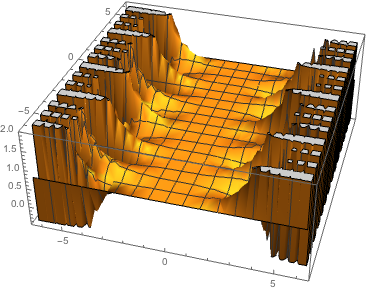
\includegraphics[scale=0.3]{lap_01_3} & 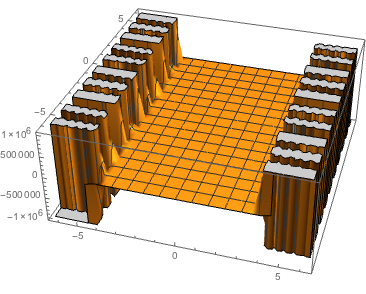
\includegraphics[scale=0.3]{lap_01_30} & 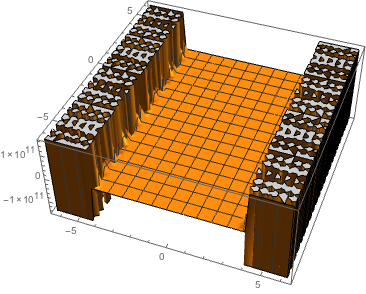
\includegraphics[scale=0.3]{lap_01_50}\\
\textit{The first 3 terms} & \textit{The first 30 terms} & \textit{The first 50 terms}
\end{tabular}
\end{center}
Plugging this infinite sum into mathematica tells us that it does not converge; the values are heading towards $\infty$ as the sum grows. We will leave our answer as a series, and we are done.
